% textidote: ignore begin
\subsection{Rejseplanen}\label{subsec:rejseplanen}
% textidote: ignore end

In Denmark, the most popular commuting planner application by far is Rejseplanen.
This application, just like Google Maps, is both available as a web and mobile application.
The app lets the traveler or commuter to enter trip starting and ending locations, which it then uses to calculate a
route using public means of transportation or as secondary options as walking routes.
When a route is calculated, the user is presented with a list-like interface from which the details of the trip can be
read; what means of transportation will be used, which lines, what the departure and arrival times are, and if there are
any special restrictions on the trip.
See Figure~\ref{fig:figure8}.

\begin{wrapfigure}{r}{0.4\textwidth}
    \begin{center}
        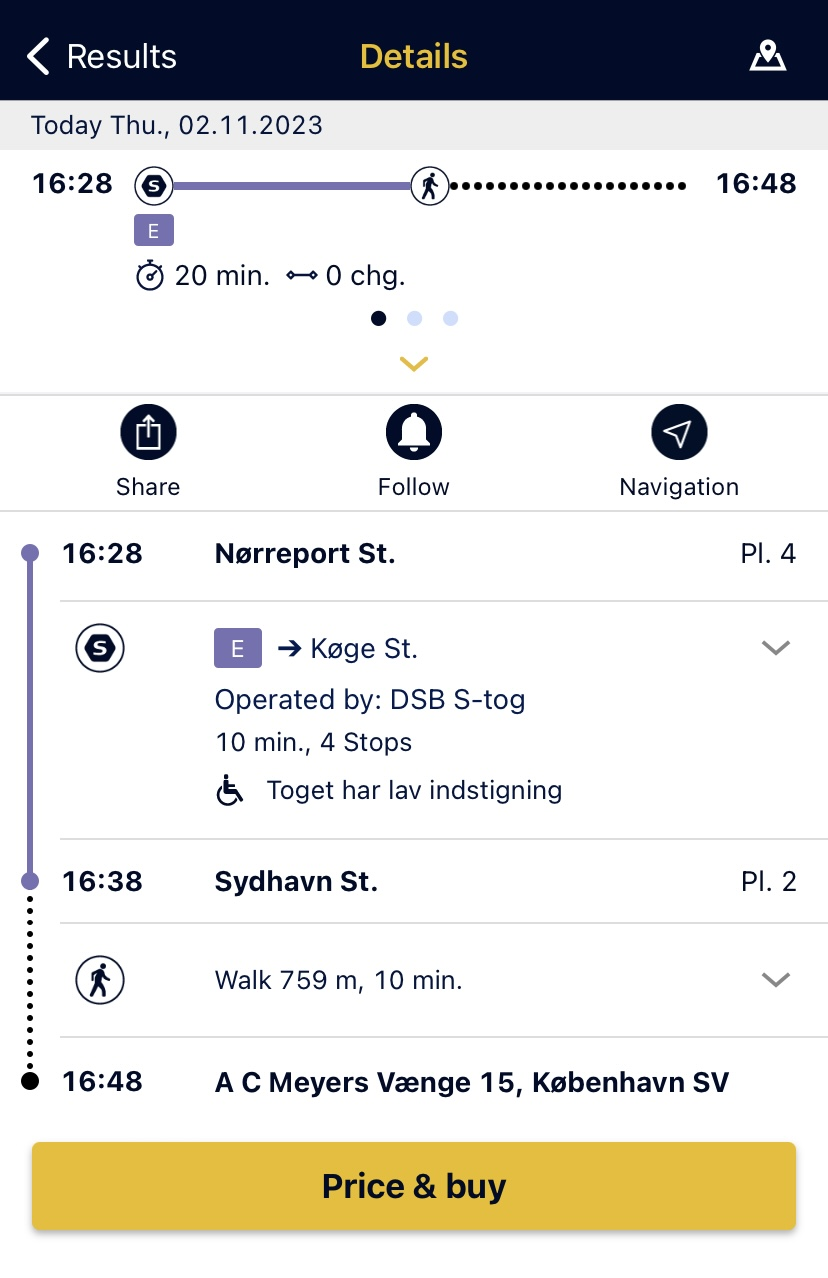
\includegraphics[width=0.3\textwidth]{rejseplanen-trip}
    \end{center}
    \caption{Rejseplanen mobile UI trip planner.}
    \label{fig:figure8}
\end{wrapfigure}

With ``Rejseplanen'', you can input your departure point and destination point to get information about the fastest,
cheapest or most convenient way to travel from point A to B using public transport.
The service provides detailed information about the departure times, transfers, expected arrival times and prices.
It also provides any additional information about the delays or canceled departures in the operation of public
transport~\cite{rejseplanen2023}.

Rejseplanen also supports ticket purchases for public transportation but ``Rejseplanen'' itself does not sell tickets
directly.
Instead, it redirects you to another website or dedicated app DOT (if installed) associated with the respective
transportation service provider.
The redirection ensures a smooth and integrated ticketing experience, allowing the users to complete their journey
planning and ticket purchase in a cohesive manner~\cite{rejseplanen2023}.

Getting the price of the trip is possible too, but in a primitive manner that doesn't consider factors such as if the
user is a tourist or a regular resident, which is an important feature since tourists might have different traveling
strategies than regular residents, and additionally tourists might not use the prepaid Rejsekort card, etc.
There is an additional option of adding your Rejsekort ID to the app, so it can calculate the trip price based on your
card plan, but even that feature is kept rather simple, possibly because the Danish transportation authorities also
released the DOT app, whose primary responsibility is exactly that: calculating trip prices and buying tickets.
See Figure~\ref{fig:figure9}.

\begin{figure}
    \centering
    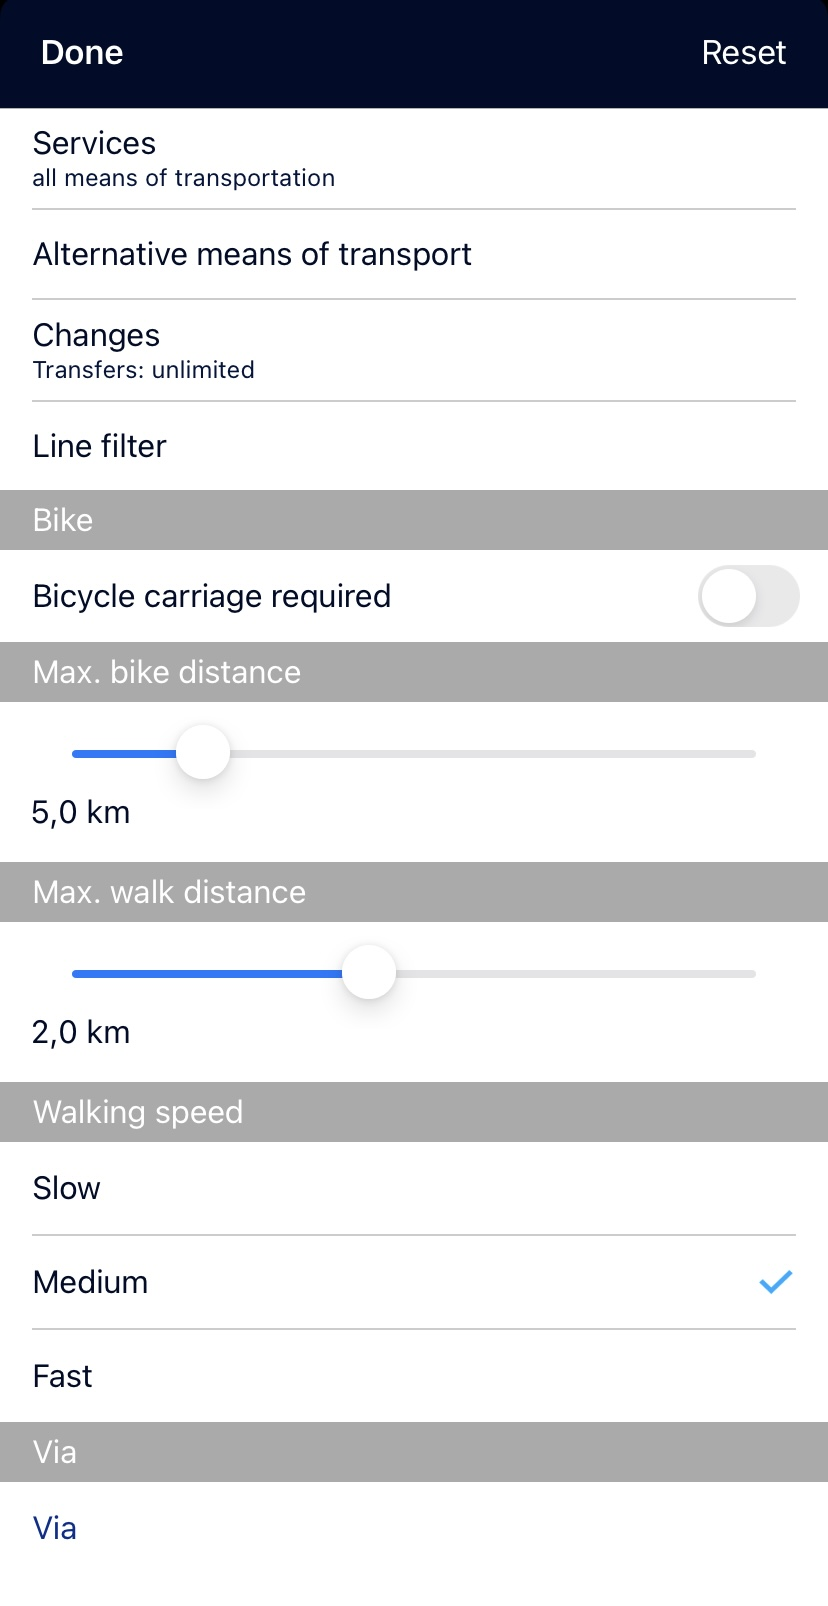
\includegraphics[width=0.5\textwidth]{rejseplanen-options}
    \caption{Rejseplanen mobile UI trip planner options.}
    \label{fig:figure9}
\end{figure}

The user can also customize the trip's parameters slightly, e.g., if it's a biking or a walking trip, what the maximum
allowed biking or walking distance should be, whether the user is a ``slow'', ``medium'' or ``fast'' walker (even though
there is no guideline for how fast exactly each of these options is), and a few additional details, but a feature that
definitely lacks is the calculation of the trip’s total \unit{CO_{2}} emissions, which is an important factor in the
modern-day world.

\subsubsection{What makes rejseplanen great?}
\begin{itemize}
    \item \textbf{Comprehensive data integration}: Rejseplanen integrates data from various transportation providers,
    thus ensuring up-to-date and accurate information.
    \item \textbf{Very efficient}: Rejseplanen provides a quick and convenient travel plan, saving time for daily
    commuters.
    \item \textbf{User-friendly}: Rejseplanen provides additional features such as filtering out specific trains or
    buses, so your route matches your personal preferences and enhancing the user experience.
\end{itemize}

In summary, ``Rejseplanen'' serves as an indispensable tool for individuals navigating Denmark's public transport system
offering a solution for journey planning, real-time updates and ticket purchases, contributing to the overall efficiency
and convenience of public transportation for commuters in the country.

% textidote: ignore begin
\subsubsection{Data sources for Rejseplanen}
% textidote: ignore end

Rejseplanen is jointly owned by DSB, Movia, Metroselskabet, NT, Midttrafik, Sydtrafik, Fynbus, and BAT\@.
As a result of its ownership by these various transportation service providers, Rejseplanen has access to the data
necessary to determine the most efficient public transport routes~\cite{rejseplanen2023}.

Rejseplanen's effectiveness in providing accurate and up-to-date public transport information is directly linked to its
access to a diverse range of data sources.
The ownership structure, with contributions from major transportation service providers in Denmark, ensures a
comprehensive and collaborative approach to gathering the necessary data for efficient journey planning.

By drawing data from these diverse data sources, ``Rejseplanen'' ensures a holistic approach to journey planning,
covering various modes of transportation and providing users with accurate, timely and relevant information for their
public transport needs.
